% ============================================================================
%  EEE3095S CS Project 2026: Serial Game Server
%  STUDENT REPORT TEMPLATE (IEEE conference format, max 10 pages incl. refs)
% ============================================================================
%
%  How to use this template
%  ------------------------
%  * Red text in [square brackets] is PLACEHOLDER text. Replace every piece of
%    it with your own words. Search the PDF for "[" before you submit.
%  * Grey boxes are GUIDANCE. They tell you what the marker looks for. Leave
%    them on while you write, then switch them off below (\guidancefalse) to
%    check your length against the 10-page limit and before you submit.
%  * Dashed boxes are PLACEHOLDER FIGURES. Replace each with your own diagram
%    (\includegraphics{figures/yourfile.pdf} or TikZ).
%  * Keep the section headings exactly as they are: they are the brief's
%    required headings, in the brief's order, and the marking guide follows
%    them. Add your own subsection headings underneath.
%  * Build:  latexmk -pdf main.tex   (or upload the folder to Overleaf).
% ============================================================================
\pdfminorversion=7
\documentclass[conference]{IEEEtran}

\usepackage[T1]{fontenc}
\usepackage{cite}
\usepackage{amsmath}
\usepackage{graphicx}
\usepackage{booktabs}
\usepackage{array}
\usepackage{xcolor}
\usepackage{listings}
\usepackage{tikz}
\usepackage[most]{tcolorbox}
\usepackage[hidelinks]{hyperref}

% ---------------------------------------------------------------- switches --
\newif\ifguidance
\guidancefalse       % <-- change to \guidancefalse to hide all guidance boxes

% ------------------------------------------------------- template helpers --
\definecolor{phred}{rgb}{0.75,0.08,0.08}
\definecolor{guidebg}{gray}{0.94}
\definecolor{guideframe}{gray}{0.55}

% Placeholder text: replace with your own.
\newcommand{\ph}[1]{\textcolor{phred}{[#1]}}

% Guidance box: what the marker expects. Hidden when \guidancefalse.
\newtcolorbox{guidebox}[1][]{
  breakable, enhanced, colback=guidebg, colframe=guideframe,
  boxrule=0.4pt, arc=1pt, left=3pt, right=3pt, top=2pt, bottom=2pt,
  fontupper=\footnotesize\sffamily, title={#1},
  fonttitle=\footnotesize\sffamily\bfseries, coltitle=black,
  colbacktitle=guidebg!80!gray, before skip=4pt, after skip=6pt}
\newenvironment{guidance}[1][Guidance]
  {\ifguidance\begin{guidebox}[#1]\else\setbox0\vbox\bgroup\fi}
  {\ifguidance\end{guidebox}\else\egroup\fi}

% Placeholder figure: dashed box with a description of what to draw.
% Usage: \figph{<height>}{<what the figure must show>}
\newcommand{\figph}[2]{%
  \begin{tikzpicture}
    \draw[dashed, phred, line width=0.6pt] (0.3pt,0) rectangle (\linewidth-0.3pt,#1);
    \node[text width=0.85\linewidth, align=center, text=phred, font=\footnotesize]
      at (0.5\linewidth,0.5*#1) {#2};
  \end{tikzpicture}}

\newcolumntype{L}[1]{>{\raggedright\arraybackslash}p{#1}}

\lstset{
  basicstyle=\fontsize{7.5pt}{8.8pt}\selectfont\ttfamily, columns=fullflexible, keepspaces=true,
  frame=tb, framerule=0.4pt, commentstyle=\color{gray}\itshape,
  keywordstyle=\bfseries, showstringspaces=false, breaklines=true,
  captionpos=b, float=tbp, floatplacement=tbp,
  aboveskip=4pt, belowskip=4pt,
}
\renewcommand{\lstlistingname}{Listing}

\begin{document}

% ---------------------------------------------------------------- title ----
\title{An Authoritative STM32 Battleship Server with a Thin PyQt6 Client and Microcontroller Heatmap AI}

\author{
\IEEEauthorblockN{Scott Faurholm (FRHSCO001)}
\IEEEauthorblockA{EEE3095S CS Project 2026, Department of Electrical Engineering\\
University of Cape Town}
}

\maketitle

\begin{abstract}
This paper presents the design, implementation, and empirical verification of an authoritative embedded game server and desktop graphical client for Battleship. The game engine is hosted on an ARM Cortex-M0 microcontroller (STM32F051R8) running bare-metal C firmware, interfaced over an asynchronous 115,200 baud UART link to a responsive Python PyQt6 desktop application. The server operates as the sole arbiter of match state, enforcing atomic two-phase fleet placement, strict turn alternating mechanics, two-stage ship sinking logic, and a deterministic integer-only probability heatmap search algorithm for autonomous on-chip artificial intelligence. Communication robustness is guaranteed through delimiter-based frame parsing, boundary saturation guards, and non-blocking inter-byte silence timeouts that clear corrupted frames within 500\,ms without blocking CPU cycles. The implementation was comprehensively validated through an automated hardware-in-the-loop test suite using pytest and pySerial, achieving 80 passing tests out of 80 across all protocol edge cases, move rejection scenarios, and AI gameplay sequences executed directly on physical microcontroller hardware.
\end{abstract}

\begin{guidance}[Before you start writing]
\begin{itemize}\setlength\itemsep{0pt}
\item \textbf{Marks} (brief, p.~6): Introduction 10, Protocol 15, Specification
  and design 15, Implementation 15, Game logic and server authority 15,
  Robustness 10, Validation 15, Conclusion 5. Video and Code links are required.
\item \textbf{Limit:} 10 pages \emph{including} references. Switch guidance off
  (\texttt{\textbackslash guidancefalse} in \texttt{main.tex}) to see your true length.
\item \textbf{Write headings that state a finding}, not just a topic, e.g.
  ``Validation runs before any state change'' rather than ``Validation''.
  Keep the section headings below as they are.
\item \textbf{Be specific}: name your mechanisms and give numbers
  (``rejects frames longer than 32 bytes''), not adjectives (``robust'',
  ``efficient'', ``significant'').
\item \textbf{Every figure, table and listing must be referred to and explained
  in the text.} Say what the reader should notice.
\item \textbf{Never present a result you did not measure.} If something is still
  untested on the board, say so.
\end{itemize}
\end{guidance}

\section{Introduction}
\label{sec:intro}

\begin{guidance}[Introduction (10 marks), about half a page]
The marker wants: the context and goal of the project; your \textbf{selected
game} and \textbf{GUI library}, with the reason for each choice; your main
\textbf{design choices}; the \textbf{task allocation} between the two of you; and
the \textbf{structure} of the report. Keep it to about half a page (brief,
p.~6). Open with the problem, not with the technology. Expand every acronym at
first use, e.g.\ ``finite-state machine (FSM)''.
\end{guidance}

In networked and serial gaming architectures, placing game logic or rule enforcement on the client exposes the system to desynchronization, packet manipulation, and cheating. If the client is trusted to report hits, misses, or board updates, state integrity cannot be guaranteed. As specified in the EEE3095S project brief~\cite{brief}, the solution is an authoritative referee model: a dedicated microcontroller owns the game state, validates every client transaction against strict game rules, and returns unambiguous evaluations across an asynchronous serial link. A fundamental property enforced throughout this design is \textbf{strict state invariance}: any request that is malformed, out-of-order, or invalid according to the current game phase is rejected immediately via an explicit negative acknowledgement (NACK), guaranteeing that internal server state remains completely uncorrupted.

To rigorously exercise this client-untrusted architecture, \textbf{Battleship} was selected over baseline games such as Tic-Tac-Toe. While Tic-Tac-Toe features full public board observability, Battleship inherently requires \textit{hidden information} (fog of war). This establishes a demanding test of server authority and secrecy: the microcontroller must maintain both players' secret fleet layouts in internal SRAM, evaluate incoming coordinates, and emit only localized outcomes (\texttt{HIT}, \texttt{MISS}, or \texttt{SUNK}) without ever leaking unhit ship coordinates until match conclusion. The PC client is built using \textbf{PyQt6}~\cite{guilib}, chosen for its robust signal-and-slot architecture, modern styling, and native multi-threading support via \texttt{QThread}. This enables a strictly thin client: all rule evaluations are prohibited on the PC, user inputs are locked pending microcontroller confirmation, and serial communication runs on an isolated background thread via pySerial~\cite{pyserial} to prevent graphical freezes during serial transfer.

Key design choices shape the system into a resilient embedded application. The firmware targeting the STM32F051 ARM Cortex-M0 is strictly modularized into protocol framing, transactional game logic, asynchronous hardware control, and an autonomous probability density heatmap artificial intelligence (AI) opponent. Framing employs newline-delimited ASCII strings protected by an inter-byte silence timeout and memory-safe boundary checks. Peripheral integration features a debounced hardware reset push-button, dual-colour turn indicators, and a dynamic five-LED fleet health bar. Finally, system correctness is verified using an automated, unattended test harness built on \texttt{pytest}~\cite{pytest} that drives the physical hardware over serial with automated port discovery.

\textbf{Project execution and task allocation.} This project was completed individually by Scott Faurholm (FRHSCO001). Consequently, all engineering deliverables---including the protocol specification, STM32F051 embedded firmware (FSM, atomic placement validation, hardware peripherals, and probability heatmap AI), the PyQt6 thin GUI client, the automated \texttt{pytest} test harness, and this report---were designed, implemented, and validated independently by the author.

\textbf{Structure.} The remainder of this report is organized as follows: Section~\ref{sec:protocol} defines the communication protocol, framing rules, command set, and departures from the reference specification. Section~\ref{sec:design} presents the system architecture, embedded FSM, and circuit schematic. Section~\ref{sec:impl} analyzes key implementation excerpts including atomic placement and the heatmap AI. Section~\ref{sec:authority} demonstrates server authority and proof of state invariance. Section~\ref{sec:robust} evaluates framing resilience, error responses, and garbage recovery. Section~\ref{sec:valid} presents automated test results and hardware validation. Finally, Section~\ref{sec:conclusion} concludes with limitations and proposed enhancements.

\section{Requirements and Message Protocol}
\label{sec:protocol}

\begin{guidance}[Requirements and message protocol (15 marks)]
Describe and diagram your \textbf{final} protocol: physical link (interface,
baud rate, frame format), \textbf{framing} (terminator, maximum frame length,
timeout), \textbf{board encoding}, the complete \textbf{command set}, and
\textbf{every response and error}. Cover new game, move, win/draw and
disconnect. Include at least one \textbf{sequence diagram}. \textbf{Highlight
every departure} from the brief's reference protocol (p.~3) and justify each
one. A reader should be able to write a compatible client from this section
alone.
\end{guidance}

\subsection{Physical Layer and Framing: Lines of at Most 64 Bytes Frame the Stream}
Communication between the PC client and the STM32F051 microcontroller occurs over a full-duplex asynchronous serial link via the \texttt{USART1} peripheral, utilizing pins \texttt{PA9} (\texttt{TX}) and \texttt{PA10} (\texttt{RX}). Signals are routed through the on-board ST-LINK Virtual COM Port (VCP) at 115200 baud with 8 data bits, no parity bit, and 1 stop bit (8N1). No hardware flow control is used.

Messages consist of printable 7-bit ASCII characters (\texttt{0x20}--\texttt{0x7E}) framed by a line-feed terminator (\texttt{\textbackslash n}, \texttt{0x0A}). To accommodate operating system and terminal differences, carriage-return characters (\texttt{\textbackslash r}, \texttt{0x0D}) are filtered upon ingestion. Input framing rules, bounds, and fault-recovery behaviours are summarized in Table~\ref{tab:framing}. The receive buffer is constrained to $\text{MAX\_FRAME\_LEN} = 64$ bytes; exceeding this limit flushes the index to zero to avoid stack corruption. To handle truncated transmissions without deadlock, an inter-byte silence timer clears partial buffers if no new bytes arrive within $\text{FRAME\_TIMEOUT} = 500\,\text{ms}$.

\begin{table}[t]
\centering
\caption{Framing rules, bounds, and fault responses.}
\label{tab:framing}
\footnotesize
\begin{tabular}{@{}L{2.8cm}L{5.2cm}@{}}
\toprule
Rule & Server Behaviour \\
\midrule
Frame Terminator & \texttt{\textbackslash n} (\texttt{0x0A}) completes frame, null-terminates string, and flags \texttt{frame\_ready = 1}. \\
Carriage Return & \texttt{\textbackslash r} (\texttt{0x0D}) is silently discarded during ingestion. \\
Max Frame Length & 64 bytes. Buffer overflow resets write index to 0 without corrupting memory. \\
Incomplete Frame & Inter-byte silence timeout (500\,ms) discards partial buffers and resets index to 0. \\
Invalid Characters & Non-ASCII or malformed headers trigger an immediate \texttt{NACK: BADCMD}. \\
\bottomrule
\end{tabular}
\end{table}

\subsection{Board and Fleet Coordinate Encoding}
The Battleship grid is configured as a $10 \times 10$ matrix with columns labeled A--J ($x \in [0, 9]$) and rows labeled 1--10 ($y \in [0, 9]$). A single coordinate is encoded as \texttt{<Col><Row>} (e.g.\ \texttt{A1}, \texttt{F7}, \texttt{J10}). Standard fleets comprise 5 orthogonal ships: Carrier (\texttt{C}, length 5), Battleship (\texttt{B}, length 4), Destroyer (\texttt{D}, length 3), Submarine (\texttt{S}, length 3), and Patrol Boat (\texttt{P}, length 2).

Fleet deployments are encoded as a canonical sequence of 10 coordinate endpoints representing the starting and ending cells of each ship in order of decreasing length:
\begin{align}
\label{eq:fleet_str}
\text{\texttt{FLEET: }} \langle P\rangle,&\langle C_S\rangle,\langle C_E\rangle,\langle B_S\rangle,\langle B_E\rangle, \nonumber\\
&\langle D_S\rangle,\langle D_E\rangle,\langle S_S\rangle,\langle S_E\rangle,\langle P_S\rangle,\langle P_E\rangle
\end{align}
For example, the deployment string \texttt{FLEET:~1,A1,A5,} \texttt{B1,B4,C1,C3,} \texttt{D1,D3,E1,E2} deploys Player~1's Carrier from A1 to A5, Battleship from B1 to B4, Destroyer from C1 to C3, Submarine from D1 to D3, and Patrol Boat from E1 to E2. 

Internally, each grid cell is stored as a single byte. Bits $0\text{x}00$--$0\text{x}05$ store the assigned \texttt{ShipType} (where 0 represents unhit water), and bit $0\text{x}80$ acts as the targeted mask. During active gameplay, board state is never broadcast in full to prevent client-side inspection. Instead, localized events (\texttt{HIT}, \texttt{MISS}, \texttt{SUNK}) are streamed, and the full layout is only retrievable post-match via \texttt{STATUS: <P>,<coords...>} to expose enemy positions on the game-over screen.

\begin{table}[t]
\centering
\caption{Command set and accepted states ($^\dagger$denotes extension).}
\label{tab:commands}
\scriptsize
\begin{tabular}{@{}L{2.2cm}L{1.9cm}L{3.9cm}@{}}
\toprule
Request & Accepted in State & Success Response \\
\midrule
\texttt{CONNECT} & Any & \texttt{OK} \\
\texttt{NEW: PVP}$^\dagger$ & \texttt{IDLE}, \texttt{GAME\_OVER} & \texttt{OK: NEW\_PVP} \\
\texttt{NEW: AI}$^\dagger$ & \texttt{IDLE}, \texttt{GAME\_OVER} & \texttt{OK: NEW\_AI} \\
\texttt{FLEET: <p>,<c>}$^\dagger$ & \texttt{SETUP} & \texttt{OK: SETUP\_P2} (P1 in PVP) \newline \texttt{OK: IN\_PROGRESS} (P2/AI) \\
\texttt{SHOOT: <p>,<xy>} & \texttt{IN\_PROGRESS} & \texttt{MISS: <opp>,<xy>} \newline \texttt{HIT: <opp>,<xy>} \newline \texttt{SUNK: <opp>,<s>,<xy1>,<xy2>} \newline \texttt{WIN: <p>,<s>,<xy1>,<xy2>} \\
\texttt{STATE: <p>} & \texttt{GAME\_OVER} & \texttt{STATUS: <p>,<fleet\_coords...>} \\
\texttt{DISCONNECT} & Any & \texttt{OK} \\
\bottomrule
\end{tabular}
\end{table}

\subsection{Command Set and Asynchronous Notifications}
Table~\ref{tab:commands} lists the complete set of accepted client commands. State transitions are strictly governed by the embedded FSM:
\begin{itemize}
    \item \textbf{\texttt{CONNECT}} / \textbf{\texttt{DISCONNECT}}: Resets internal variables, halts LED blinking, and establishes an active session in \texttt{STATE\_IDLE}.
    \item \textbf{\texttt{NEW: PVP}} / \textbf{\texttt{NEW: AI}}: Clears previous grid buffers and initiates fleet deployment (\texttt{STATE\_SETUP}). \texttt{NEW: AI} additionally seeds the pseudo-random generator via \texttt{HAL\_GetTick() $\oplus$ SysTick->VAL}.
    \item \textbf{\texttt{FLEET}}: Validates all 5 ships in temporary storage. If valid, locks the placement into memory. In AI mode, the microcontroller immediately deploys its own fleet and advances to \texttt{STATE\_IN\_PROGRESS}.
    \item \textbf{\texttt{SHOOT}}: Evaluates target coordinates. If valid, the target cell is marked, turn counters update, and health is adjusted. In AI mode, the MCU immediately executes a counter-attack and appends its response.
    \item \textbf{Asynchronous Hardware Reset}: Pressing the on-board user button (\texttt{PA0}) triggers a debounced interrupt, returns the server to \texttt{STATE\_IDLE}, and transmits \texttt{EVENT: RESET} to force the GUI client to the main menu.
\end{itemize}

\subsection{Error Responses and Strict Validation Precedence}
The server follows a deterministic, hierarchical error evaluation sequence for every incoming command, ensuring predictable responses:
\begin{enumerate}
    \item \textbf{Framing Check}: Overlength frames and framing timeouts clear the buffer without generating a reply.
    \item \textbf{Syntax and Parameter Parsing}: Malformed command strings, missing delimiters, out-of-range player IDs ($\ne 1, 2$), or unparseable coordinate tokens fail parsing and yield \texttt{NACK: BADCMD}.
    \item \textbf{State Machine Feasibility}: Commands sent during an inappropriate state (e.g.\ \texttt{SHOOT} before fleet deployment) yield \texttt{NACK: NOGAME} or \texttt{NACK: OUT\_OF\_STATE,<state>}.
    \item \textbf{Turn Enforcement}: Commands submitted by the inactive player yield \texttt{NACK: NOTURN}.
    \item \textbf{Geometry and Bounds Checks}: Ship placements that are diagonal, out-of-grid, or mismatched in length yield \texttt{NACK: BADCOORDS,<ship>}.
    \item \textbf{Overlap and Duplicate Checks}: Ship placements colliding with existing vessels yield \texttt{NACK: OCCUPIED,<ship>,<overlap>}. Targeted shots hitting an already-fired cell yield \texttt{NACK: REPEAT}.
\end{enumerate}
Table~\ref{tab:errors} outlines every error code and its state invariant guarantee.

\begin{table}[t]
\centering
\caption{Error responses, emission criteria, and state guarantees.}
\label{tab:errors}
\footnotesize
\begin{tabular}{@{}L{2.6cm}L{5.4cm}@{}}
\toprule
Error Response & Trigger Condition and State Guarantee \\
\midrule
\texttt{NACK: BADCMD} & Header unrecognised or parameters syntactically invalid. State unmodified. \\
\texttt{NACK: NOGAME} & Action received while in \texttt{STATE\_IDLE}. State unmodified. \\
\texttt{NACK: OUT\_OF\_STATE} & Command not permitted in current FSM phase (e.g.\ firing in setup). State unmodified. \\
\texttt{NACK: NOTURN} & Player ID does not match \texttt{current\_turn}. Turn remains with active player. \\
\texttt{NACK: BADCOORDS} & Ship is diagonal, off-board, or wrong length; or shot out-of-bounds. State unmodified. \\
\texttt{NACK: OCCUPIED} & Ship placement overlaps an already positioned ship. Entire fleet placement aborted. \\
\texttt{NACK: REPEAT} & Target cell already fired upon (bit $0\text{x}80$ set). Turn is preserved. \\
\bottomrule
\end{tabular}
\end{table}

\subsection{Departures from the Reference Protocol}
Several justified departures from the brief's Tic-Tac-Toe reference protocol (brief, p.~3) were implemented:
\begin{itemize}
    \item \textbf{Event-Based Outcomes vs.\ Board Broadcasting}: The reference protocol returns the entire board state on each move (\texttt{OK:BOARD:<chars>}). In Battleship, transmitting both grids would defeat the game's hidden-information premise. The server instead emits targeted events (\texttt{HIT}, \texttt{MISS}, \texttt{SUNK}), and only exposes the opponent's grid upon match completion.
    \item \textbf{Dedicated Setup Phase (\texttt{STATE\_SETUP})}: Battleship requires deploying multi-cell fleets prior to combat. The \texttt{FLEET} command performs atomic validation of all 5 ships before entering combat.
    \item \textbf{Diagnostic Rejection Codes}: Generic rejections were extended with contextual tokens (e.g.\ \texttt{NACK: OCCUPIED,C,B} identifies Carrier-Battleship overlap; \texttt{NACK: REPEAT} flags re-fired cells), enabling rich GUI feedback.
    \item \textbf{Absence of Draws}: In sequential Battleship with 17 finite ship cells across a $10 \times 10$ grid, fleet annihilation guarantees a definitive victor, making \texttt{DRAW} unreachable.
\end{itemize}

\begin{figure}[t]
\centering
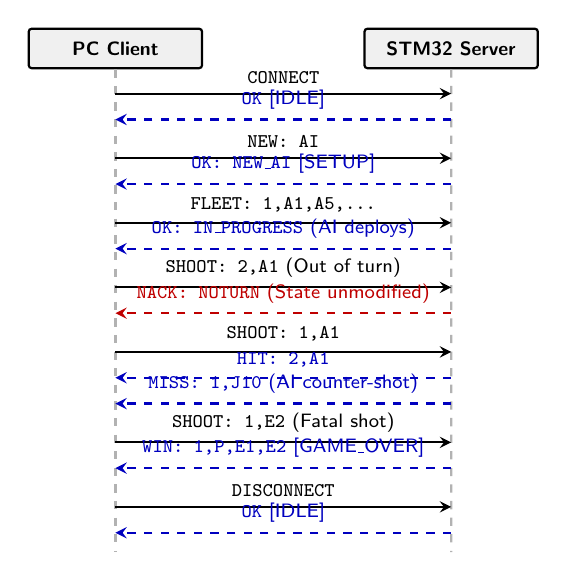
\begin{tikzpicture}[
    scale=0.82, every node/.style={font=\scriptsize\sffamily},
    lifeline/.style={thick, dashed, gray!60},
    msg/.style={->, >=stealth, thick},
    reply/.style={->, >=stealth, thick, dashed, blue!75!black},
    nack/.style={->, >=stealth, thick, dashed, red!75!black},
    box/.style={draw, thick, fill=gray!12, rounded corners=1pt, minimum width=2.2cm, minimum height=0.5cm}
]
    % Entities
    \node[box] (cli) at (0, 0) {\textbf{PC Client}};
    \node[box] (stm) at (5.2, 0) {\textbf{STM32 Server}};
    
    % Lifelines
    \draw[lifeline] (cli) -- (0, -7.8);
    \draw[lifeline] (stm) -- (5.2, -7.8);
    
    % Messages
    \draw[msg] (0, -0.7) -- node[above] {\texttt{CONNECT}} (5.2, -0.7);
    \draw[reply] (5.2, -1.1) -- node[above] {\texttt{OK} [IDLE]} (0, -1.1);
    
    \draw[msg] (0, -1.7) -- node[above] {\texttt{NEW: AI}} (5.2, -1.7);
    \draw[reply] (5.2, -2.1) -- node[above] {\texttt{OK: NEW\_AI} [SETUP]} (0, -2.1);
    
    \draw[msg] (0, -2.7) -- node[above] {\texttt{FLEET: 1,A1,A5,...}} (5.2, -2.7);
    \draw[reply] (5.2, -3.1) -- node[above] {\texttt{OK: IN\_PROGRESS} (AI deploys)} (0, -3.1);
    
    % Rejected Move
    \draw[msg] (0, -3.7) -- node[above] {\texttt{SHOOT: 2,A1} (Out of turn)} (5.2, -3.7);
    \draw[nack] (5.2, -4.1) -- node[above] {\textbf{\texttt{NACK: NOTURN}} (State unmodified)} (0, -4.1);
    
    % Combat Exchange
    \draw[msg] (0, -4.7) -- node[above] {\texttt{SHOOT: 1,A1}} (5.2, -4.7);
    \draw[reply] (5.2, -5.1) -- node[above] {\texttt{HIT: 2,A1}} (0, -5.1);
    \draw[reply] (5.2, -5.5) -- node[above] {\texttt{MISS: 1,J10} (AI counter-shot)} (0, -5.5);
    
    % Terminal Shot
    \draw[msg] (0, -6.1) -- node[above] {\texttt{SHOOT: 1,E2} (Fatal shot)} (5.2, -6.1);
    \draw[reply] (5.2, -6.5) -- node[above] {\texttt{WIN: 1,P,E1,E2} [GAME\_OVER]} (0, -6.5);
    
    % Teardown
    \draw[msg] (0, -7.1) -- node[above] {\texttt{DISCONNECT}} (5.2, -7.1);
    \draw[reply] (5.2, -7.5) -- node[above] {\texttt{OK} [IDLE]} (0, -7.5);
\end{tikzpicture}
\caption{Protocol sequence diagram showing connection, fleet deployment, out-of-turn rejection, combat exchange with AI retaliation, and terminal win resolution.}
\label{fig:sequence}
\end{figure}

\section{Specification and Design}
\label{sec:design}

\begin{guidance}[Specification and design (15 marks)]
Required (brief, A.3--A.5): an \textbf{embedded server FSM} covering IDLE,
IN\_PROGRESS, GAME\_OVER \textbf{and the move-validation branch}; a
\textbf{flowchart of the GUI application}; and a \textbf{circuit diagram} of the
STM-to-PC UART connection, with the on-board button and LED behaviour labelled.
Diagrams may be at function level. Explain \textbf{why} responsibilities sit on
the server or the client. Draw diagrams in a tool that exports vector PDF
(draw.io, TikZ, Mermaid) and check that every label is readable when printed.
\end{guidance}

\subsection{System Architecture and Separation of Concerns}
The system enforces a clean client-server divide designed around a zero-trust model: the PC client is treated as an untrusted rendering terminal, while the STM32F051 microcontroller functions as the authoritative arbiter. Table~\ref{tab:responsibilities} summarizes the allocation of responsibilities between the two domains.

The embedded firmware is decoupled into four modular subsystems:
\begin{enumerate}
    \item \textbf{Protocol Framing (\texttt{protocol.c})}: Ingests raw UART bytes via interrupt, validates frame boundaries and character sets, enforces inter-byte timeouts, and formats outbound ASCII packets.
    \item \textbf{Game Logic and FSM (\texttt{battleship.c})}: Maintains the single source of truth for grid state, evaluates move validity, coordinates atomic fleet placement, tracks fleet damage, and dictates state transitions.
    \item \textbf{Peripheral Hardware (\texttt{hardware.c})}: Manages low-level GPIO operations, button debouncing, LED health bar representation, and turn indicators.
    \item \textbf{Probability Heatmap AI (\texttt{ai.c})}: Generates legal fleet placements and autonomous targeting coordinates directly on the Cortex-M0.
\end{enumerate}

Conversely, the PC application is strictly decoupled from game rules. The GUI captures raw mouse clicks, translates them into coordinate strings, and transmits them over UART. The client cannot locally mark a cell as hit, miss, or sunken, nor can it advance turns. All interface mutations occur solely in response to authoritative microcontroller confirmations.

\begin{table}[t]
\centering
\caption{Allocation of responsibilities between PC and STM32.}
\label{tab:responsibilities}
\footnotesize
\begin{tabular}{@{}L{2.4cm}L{2.7cm}L{2.9cm}@{}}
\toprule
Domain & STM32 Server & PC GUI Client \\
\midrule
Fleet Layouts & Authoritative storage in internal SRAM (secret). & Local cache populated strictly upon server confirmation. \\
Turn Tracking & Authoritative counter (\texttt{current\_turn}). & Reflects server-directed turn state; locks inputs out-of-turn. \\
Move Legality & Validates syntax, bounds, turn, and prior hits. & Forwards raw click; cannot evaluate legality. \\
Hit / Miss / Win & Computes cell intersection and damage. & Renders sprites according to received server token. \\
Hardware I/O & GPIO LEDs, debounced push-button, USART. & Virtual COM Port communication via background thread. \\
\bottomrule
\end{tabular}
\end{table}

\begin{figure*}[t]
\centering
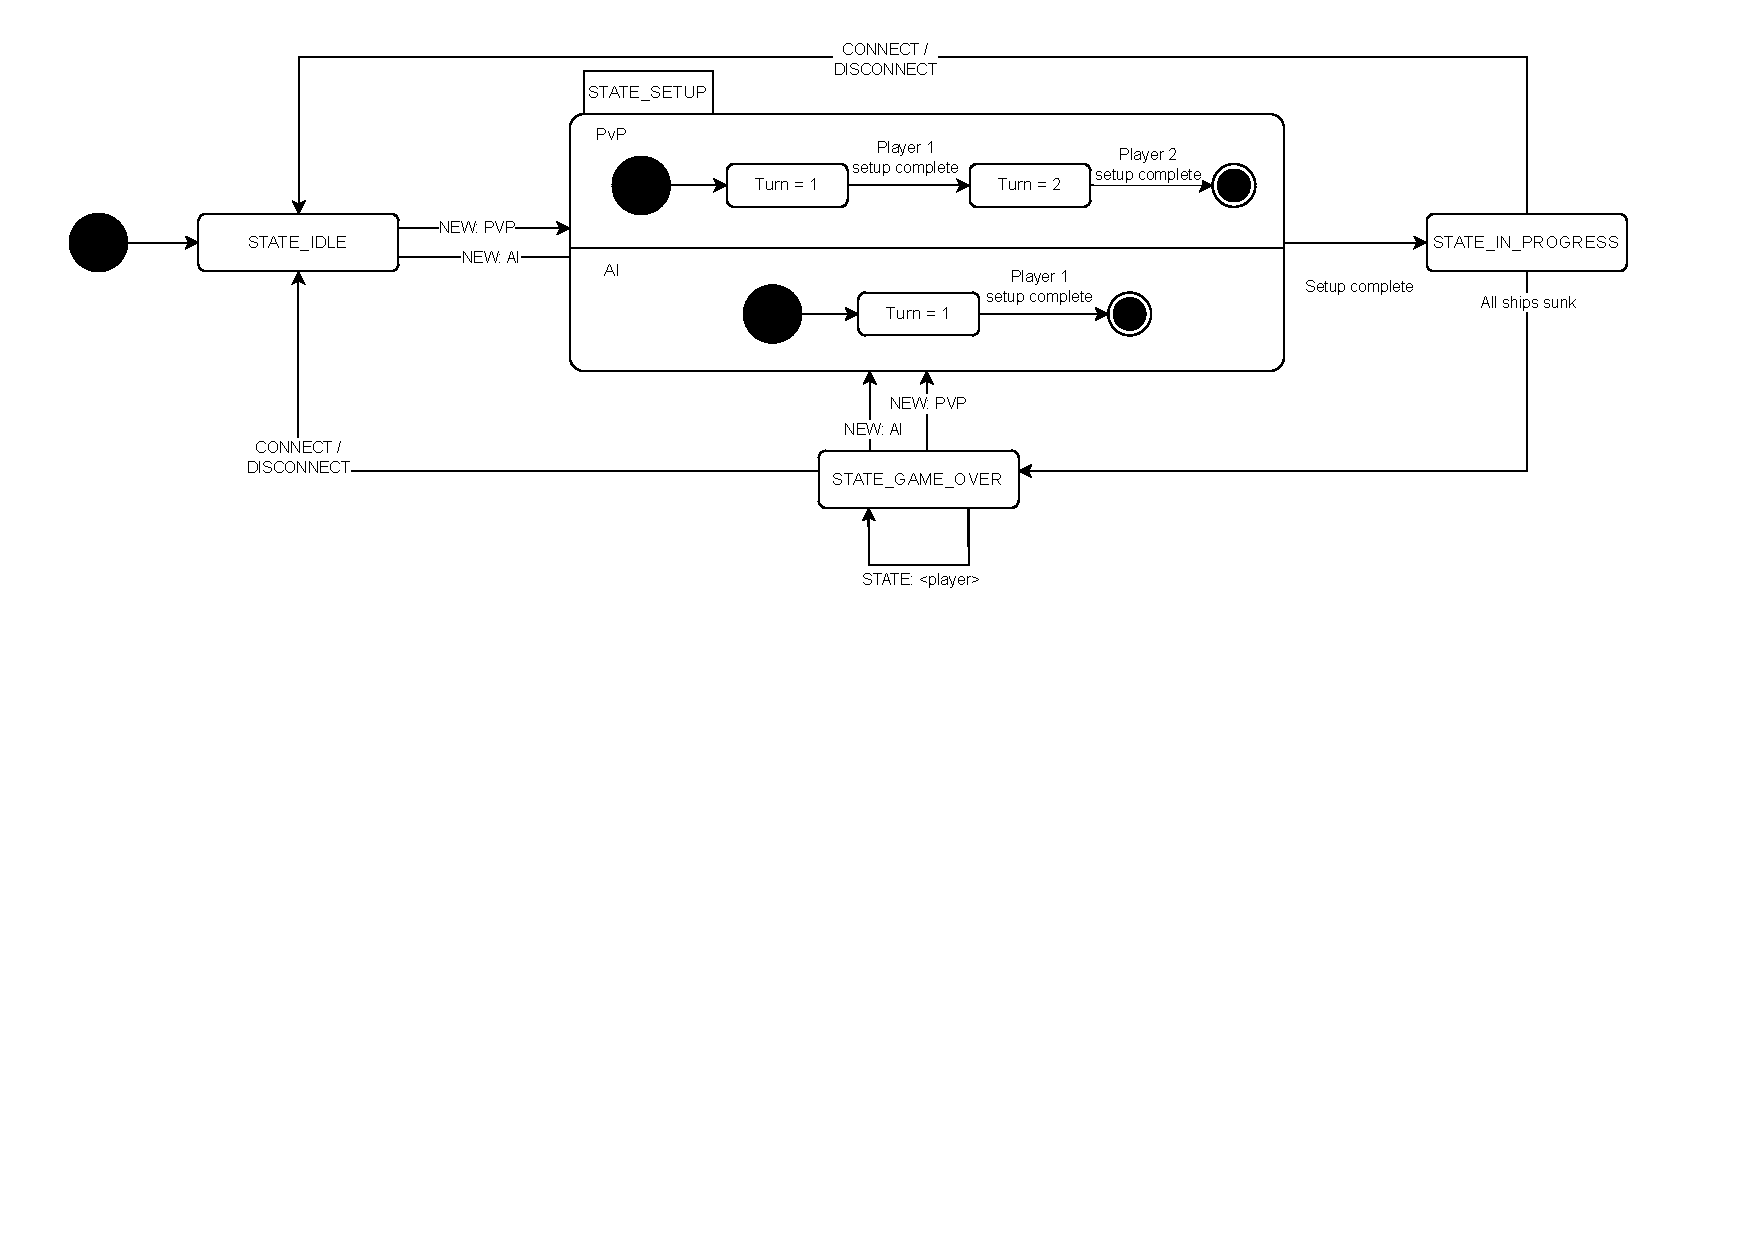
\includegraphics[width=0.82\textwidth]{figures/FSM_diagram.pdf}
\caption{Embedded server finite-state machine (FSM) showing top-level state transitions and the move-validation branch. Any failed check exits immediately with a specific NACK, leaving the grid state completely unmodified.}
\label{fig:fsm}
\end{figure*}

\subsection{Embedded Server Finite-State Machine}
The embedded server FSM (Fig.~\ref{fig:fsm}) implements four operational states and a deterministic validation tree:
\begin{itemize}
    \item \textbf{\texttt{STATE\_IDLE}}: Bootstrapping state. Configures clocks, peripherals, and interrupt lines. Ignores combat actions with \texttt{NACK: NOGAME}. Acknowledges \texttt{CONNECT} and initializes session variables. Transition to \texttt{STATE\_SETUP} occurs upon receiving \texttt{NEW: PVP} or \texttt{NEW: AI}.
    \item \textbf{\texttt{STATE\_SETUP}}: Enforces atomic fleet positioning via \texttt{FLEET: <p>,<coords...>}. In Player-vs-Player (PVP) mode, Player~1 placement yields \texttt{OK: SETUP\_P2} and advances \texttt{current\_turn = 2}; Player~2 placement completes setup and advances to \texttt{STATE\_IN\_PROGRESS}. In AI mode, Player~1 placement immediately triggers on-board AI fleet generation, initializes the AI hunt/target engine, and transitions directly to combat.
    \item \textbf{\texttt{STATE\_IN\_PROGRESS}}: Active gameplay loop. As illustrated in Fig.~\ref{fig:fsm}, every incoming \texttt{SHOOT} command passes through a sequential validation pipeline:
    \begin{enumerate}
        \item \textit{Turn Lock}: Ensures the acting player corresponds to \texttt{current\_turn}, guarding against out-of-order execution (\texttt{NACK: NOTURN}).
        \item \textit{Coordinate Range}: Validates that row and column indices reside strictly within $[0, 9]$ (\texttt{NACK: BADCOORDS}).
        \item \textit{Duplicate Shot}: Inspects bit $0\text{x}80$ of the target cell. If already set, rejects duplicate firing without consuming the player's turn (\texttt{NACK: REPEAT}).
        \item \textit{Damage Evaluation}: Marks the cell with bit $0\text{x}80$. If the cell contains \texttt{SHIP\_NONE}, emits \texttt{MISS} and toggles turns. If a vessel is present, increments damage counters, emitting \texttt{HIT} or \texttt{SUNK}.
        \item \textit{Terminal Condition}: Sinking the 5th fleet vessel satisfies the win predicate, broadcasting \texttt{WIN} and entering \texttt{STATE\_GAME\_OVER}.
    \end{enumerate}
    \item \textbf{\texttt{STATE\_GAME\_OVER}}: Combat is permanently halted. Any subsequent shot yields \texttt{NACK: OUT\_OF\_STATE,GAME\_OVER}. Status LEDs alternate in a 250\,ms blinking pattern. Responds to \texttt{STATE: 2} by returning the full AI fleet to populate the end-game review screen, or accepts \texttt{NEW} to commence a new match.
\end{itemize}

\begin{figure}[t]
\centering
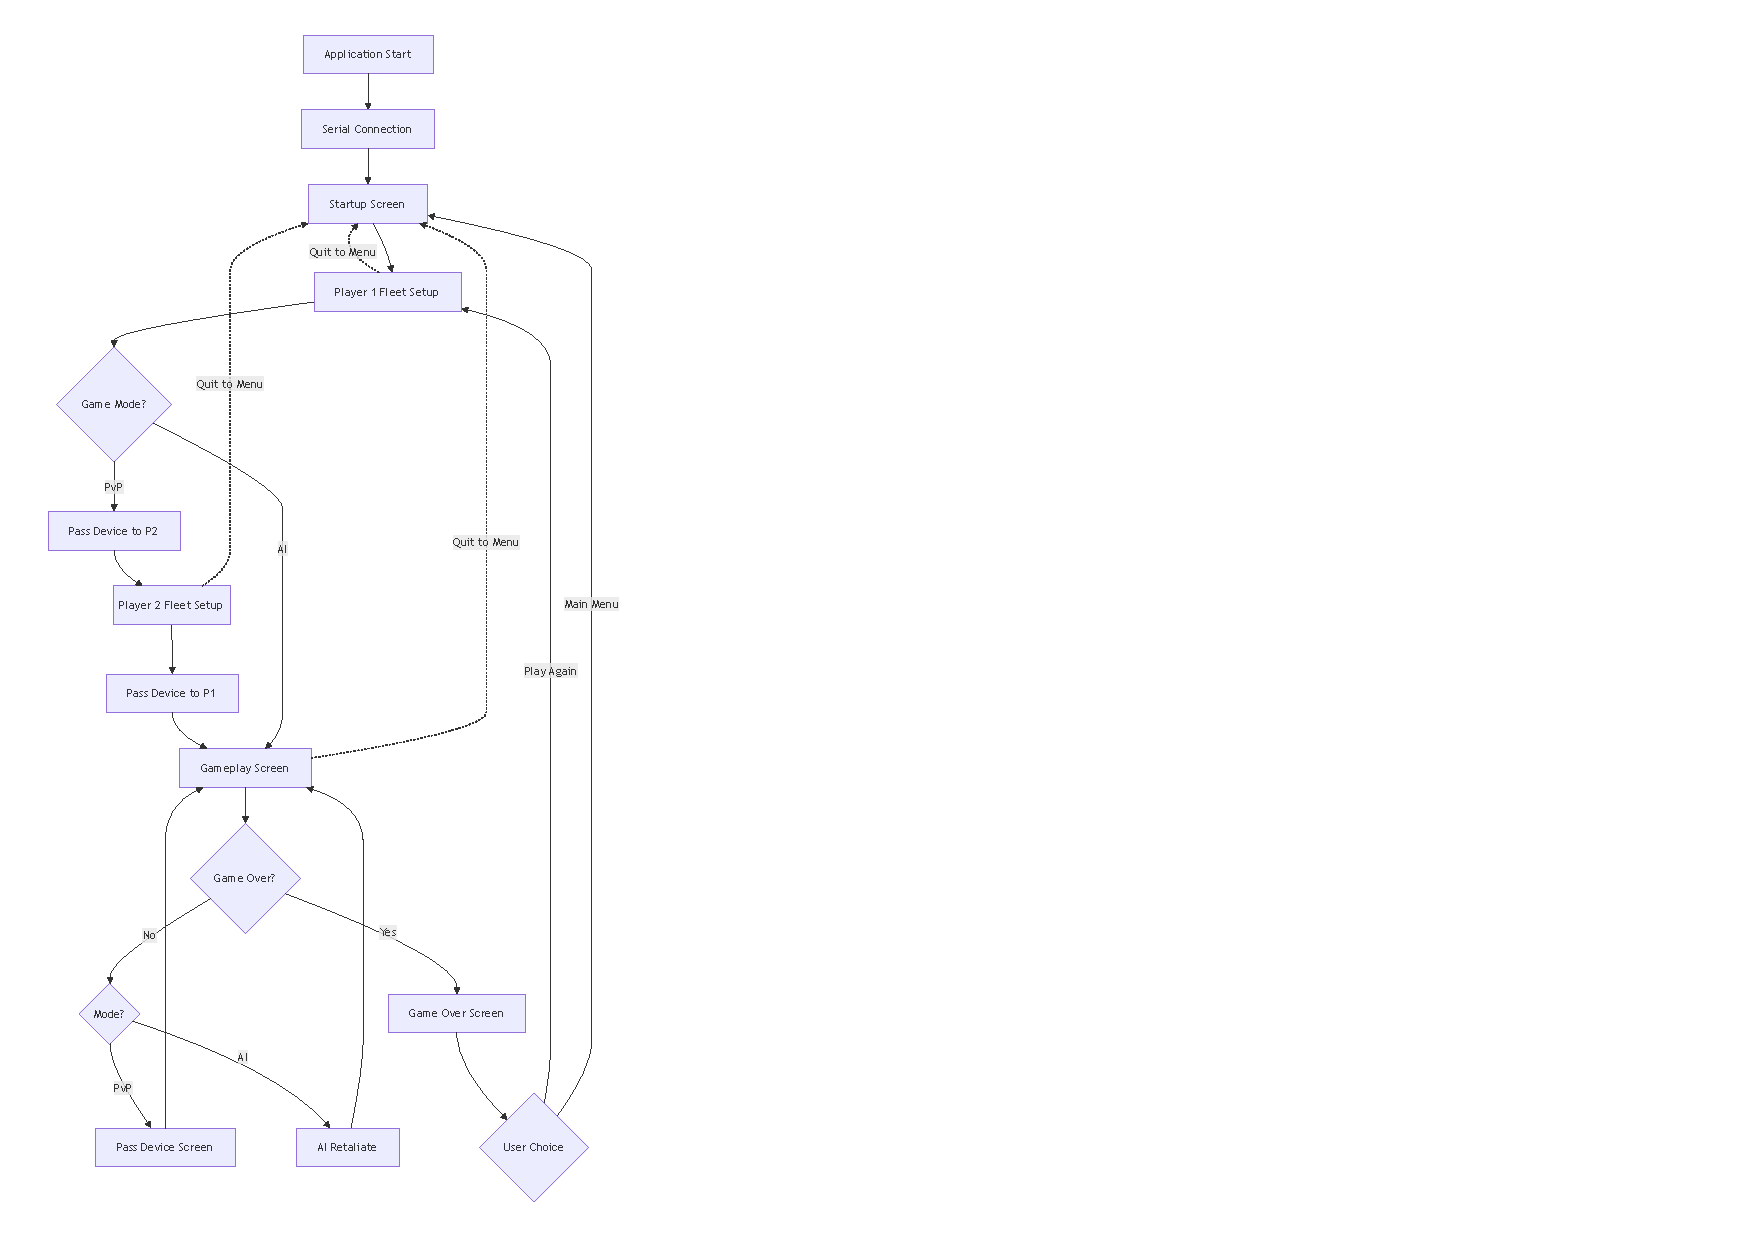
\includegraphics[width=0.88\columnwidth]{figures/GUI_diagram.pdf}
\caption{PC GUI client application flowchart illustrating connection discovery, fleet deployment pathways, turn sequencing, and game-over resolution.}
\label{fig:gui}
\end{figure}

\subsection{PC GUI Client Flowchart and Concurrency Architecture}
The PC client application architecture (Fig.~\ref{fig:gui}) is structured as a finite stack of views managed by a central \texttt{QStackedWidget} in \texttt{MainWindow}:
\begin{enumerate}
    \item \textbf{Startup and Auto-Discovery}: On launch, \texttt{SerialWorker} queries all system COM ports. It scans hardware description strings for ST-LINK and standard USB-to-UART bridge signatures, connecting automatically without requiring manual port entry.
    \item \textbf{Fleet Setup and Masking}: Players position ships using visual snap-to-grid controls. In PVP mode, to prevent screen-peeking during local hotseat play, the application inserts a \texttt{PassDeviceScreen} between Player~1 and Player~2 setup phases, ensuring fleet layouts remain concealed.
    \item \textbf{Gameplay Loop}: During active play, the GUI renders two separate grids: the active player's secret \textit{Home Fleet} (showing ships and incoming enemy fire) and the \textit{Target Radar} (displaying confirmed shots). Clicking a radar cell immediately locks the UI, transmits the \texttt{SHOOT} command, and awaits microcontroller resolution.
    \item \textbf{Game Over and Fleet Reveal}: Upon receiving \texttt{WIN}, the client queries the server for the opponent's true coordinates (\texttt{STATE: 2}), transitioning to the \texttt{GameOverScreen} where sunken vessels and unhit enemy ships are fully revealed.
\end{enumerate}

To ensure complete responsiveness, all serial communications are executed asynchronously within a dedicated \texttt{QThread} subclass (\texttt{SerialWorker}). Communication between the worker thread and the GUI relies exclusively on thread-safe Qt signals and slots:
\begin{itemize}
    \item Outbound frames are placed into a thread-safe FIFO queue (\texttt{queue.Queue}) via the slot \texttt{send\_command()}, where the background thread drains and transmits bytes over UART.
    \item Inbound lines are read non-blockingly via \texttt{readline()}, stripped of delimiters, and emitted through the \texttt{message\_received(str)} signal directly into the main thread router \texttt{handle\_server\_response()}.
\end{itemize}
This threading design guarantees that serial transmission latencies or hardware timeouts never block the main Qt event loop, preventing UI freezing or frame dropping.

\begin{figure}[t]
\centering
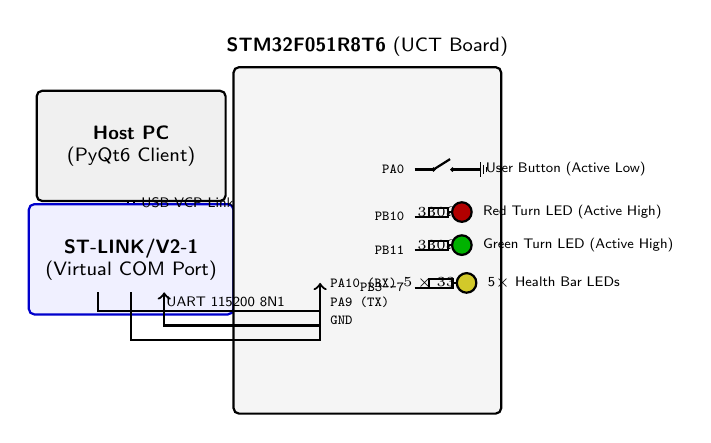
\begin{tikzpicture}[
    scale=0.60, every node/.style={font=\scriptsize\sffamily},
    chip/.style={draw=black, thick, fill=gray!8, rounded corners=2pt, minimum width=3.4cm, minimum height=4.4cm, align=center},
    pcbox/.style={draw=black, thick, fill=gray!12, rounded corners=2pt, minimum width=2.4cm, minimum height=1.4cm, align=center},
    pin/.style={font=\tiny\ttfamily},
    wire/.style={thick}
]
    % PC Block
    \node[pcbox] (pc) at (0, 2.4) {\textbf{Host PC}\\\scriptsize(PyQt6 Client)};

    % ST-LINK Block
    \node[draw=blue!80!black, thick, fill=blue!6, rounded corners=2pt, minimum width=2.6cm, minimum height=1.4cm, align=center] (stlink) at (0, 0) {\textbf{ST-LINK/V2-1}\\\scriptsize(Virtual COM Port)};

    % STM32F051 Block
    \node[chip] (stm) at (5.0, 0.4) {};
    \node[above] at (stm.north) {\textbf{STM32F051R8T6} (UCT Board)};

    % USB Connection
    \draw[wire, double, double distance=1.5pt] (pc) -- node[right, font=\tiny\sffamily] {USB VCP Link} (stlink);

    % UART Pins between ST-LINK and STM32
    \draw[wire, ->] (-0.7, -0.7) -- ++(0, -0.4) -| (4.0, -0.5) node[pin, right] {PA10 (RX)};
    \draw[wire, <-] (0.7, -0.7) -- ++(0, -0.7) -| (4.0, -0.9) node[pin, right] {PA9 (TX)};
    \draw[wire] (0, -0.7) -- ++(0, -1.0) -| (4.0, -1.3) node[pin, right] {GND};

    \node[font=\tiny\sffamily] at (2.0, -0.9) {UART 115200 8N1};

    % Peripherals on STM32
    % Reset Button
    \draw[wire] (6.0, 1.9) node[pin, left] {PA0} -- ++(0.4, 0) coordinate (b1);
    \draw[wire] (b1) ++(0.4, 0) coordinate (b2) -- ++(0.4, 0) coordinate (bgnd);
    \draw[wire] (b1) -- ++(0.35, 0.22);
    \filldraw (b1) circle (1pt) (b2) circle (1pt);
    \node[font=\tiny\sffamily, right] at (7.3, 1.9) {User Button (Active Low)};
    % Ground
    \draw[wire] (bgnd) -- ++(0.2, 0) coordinate (g1);
    \draw (g1) ++(0, 0.15) -- ++(0, -0.3);
    \draw (g1) ++(0.06, 0.10) -- ++(0, -0.2);
    \draw (g1) ++(0.12, 0.05) -- ++(0, -0.1);

    % Status LEDs
    \draw[wire] (6.0, 0.9) node[pin, left] {PB10} -- ++(0.3, 0) rectangle ++(0.4, 0.18);
    \node[font=\tiny] at (6.5, 1.0) {330$\Omega$};
    \draw[wire] (6.7, 1.0) -- ++(0.3, 0) node[circle, draw, fill=red!70!black, inner sep=2.5pt, label=right:\tiny Red Turn LED (Active High)] {};

    \draw[wire] (6.0, 0.2) node[pin, left] {PB11} -- ++(0.3, 0) rectangle ++(0.4, 0.18);
    \node[font=\tiny] at (6.5, 0.3) {330$\Omega$};
    \draw[wire] (6.7, 0.3) -- ++(0.3, 0) node[circle, draw, fill=green!70!black, inner sep=2.5pt, label=right:\tiny Green Turn LED (Active High)] {};

    % Health Bar LEDs
    \draw[wire] (6.0, -0.6) node[pin, left] {PB3--7} -- ++(0.3, 0) rectangle ++(0.5, 0.18);
    \node[font=\tiny] at (6.55, -0.5) {$5\times330\Omega$};
    \draw[wire] (6.8, -0.5) -- ++(0.3, 0) node[circle, draw, fill=yellow!80!black, inner sep=2.5pt, label=right:\tiny 5$\times$ Health Bar LEDs] {};
\end{tikzpicture}
\caption{System circuit diagram showing the physical UART interface routed through the on-board ST-LINK Virtual COM Port, the debounced user push-button on \texttt{PA0}, and GPIO status and health bar indicator LEDs.}
\label{fig:circuit}
\end{figure}

\subsection{Circuit Topology and Peripheral Integration}
Fig.~\ref{fig:circuit} illustrates the physical circuit topology connecting the STM32F051R8T6 microcontroller to the host PC and external user indicators:
\begin{itemize}
    \item \textbf{Host Serial Interface}: The microcontroller's \texttt{USART1} pins (\texttt{PA9} TX and \texttt{PA10} RX) route directly to the embedded ST-LINK/V2-1 interface on the Discovery board. The ST-LINK bridge enumerates as a USB Virtual COM Port (VCP) on the host machine, establishing bi-directional serial transfer at 115200 baud without requiring external USB-to-UART breakout boards or level shifters.
    \item \textbf{User Reset Button (\texttt{PA0})}: Connected to the momentary push-button. Configured in software as a floating input with an internal pull-up resistor (\texttt{GPIO\_PULLUP}). Pressing the button pulls \texttt{PA0} to ground. Software debouncing in \texttt{hardware.c} requires the input to remain stable low across a 50\,ms timing threshold before emitting \texttt{EVENT: RESET} and re-initializing game state.
    \item \textbf{Status and Turn Indicators (\texttt{PB10}, \texttt{PB11})}: Configured as active-high push-pull outputs driving visual indicator LEDs through current-limiting resistors. In \texttt{STATE\_IN\_PROGRESS}, \texttt{PB11} (Green) illuminates when Player~1 is active, while \texttt{PB10} (Red) illuminates during Player~2 or AI turns. In \texttt{STATE\_GAME\_OVER}, the winning player's LED blinks at a 250\,ms cadence.
    \item \textbf{Dynamic Health Bar (\texttt{PB3}--\texttt{PB7})}: A five-LED bar graph reflects the current number of surviving ships in the active player's fleet (or Player~1's health in AI mode). As ships are destroyed, corresponding LEDs are systematically extinguished, providing direct hardware feedback of combat progression.
\end{itemize}

\section{Implementation}
\label{sec:impl}

\begin{guidance}[Implementation (15 marks)]
Choose \textbf{3 to 5 short code excerpts} that were \textbf{not straightforward}
to write, and explain each: what problem it solves, why you wrote it this way,
and what would go wrong with the obvious alternative. Good candidates:
receiving bytes in an interrupt and handing them to the main loop; the frame
assembler with timeout and oversize handling; non-blocking button debounce;
keeping the GUI responsive; separating unsolicited messages from replies.
Keep each listing short (10--25 lines) and narrow enough for one column; trim
comments and boilerplate, and say that you did. Do not paste whole files.
\end{guidance}

\subsection{Interrupt-Driven Frame Assembler and Inter-Byte Silence Timeout}
Assembling asynchronous serial streams on microcontrollers without operating system services poses two key hazards: buffer overruns caused by oversized or garbage packets, and deadlocks caused by stalled transmissions. The naive solution of polling UART bytes with \texttt{HAL\_UART\_Receive()}~\cite{um1785} blocks the main thread, starving button debouncing and LED timing. Conversely, accumulating frames inside a fixed buffer without timing bounds risks corruption if a packet is truncated.

Listing~\ref{lst:proto_rx} illustrates the two-tiered solution. Ingestion executes inside the UART receive complete interrupt callback (\texttt{USART1\_IRQHandler}), which passes incoming bytes to \texttt{Proto\_ProcessByte()}. Every ingested byte refreshes \texttt{last\_rx\_time} to the current millisecond tick (\texttt{HAL\_GetTick()}), establishing an inter-byte silence detector. If the buffer exceeds $\text{MAX\_FRAME\_LEN} - 1$ (63 bytes) before a newline arrives, the write index is reset immediately. Concurrently, the non-blocking main loop checks whether $\text{FRAME\_TIMEOUT} = 500\,\text{ms}$ has elapsed since the last byte; if true, any partial frame is safely purged.

\begin{lstlisting}[language=C, caption={Interrupt ingestion and inter-byte timeout (\texttt{protocol.c}, \texttt{main.c}).}, label=lst:proto_rx]
/* protocol.c - Ingest byte from UART ISR */
void Proto_ProcessByte(uint8_t byte) {
  last_rx_time = HAL_GetTick(); /* Refresh silence timestamp */
  if (byte == '\r') return;
  if (byte == '\n') {
    rx_buffer[rx_index] = '\0';
    frame_ready = 1; rx_index = 0; return;
  }
  if (rx_index < (MAX_FRAME_LEN - 1)) {
    rx_buffer[rx_index++] = (char)byte;
  } else { rx_index = 0; } /* Saturation flush */
}
/* main.c - Non-blocking silence timeout */
if (rx_index > 0 && (now - last_rx_time > FRAME_TIMEOUT)) {
  rx_index = 0; last_rx_time = now; /* Flush stalled fragment */
}
\end{lstlisting}

\subsection{Transactional Two-Phase Commit for Fleet Deployment}
In Battleship, a player deploys five multi-cell vessels simultaneously. Each vessel must satisfy strict geometric invariants: exact length ($5, 4, 3, 3, 2$), strict grid confinement ($x, y \in [0, 9]$), perfect orthogonality (no diagonals), and zero overlap with any other vessel. If validation were executed directly against the live game board, an error encountered on the fourth or fifth ship would leave the board in a corrupt, partially placed state requiring complex rollback logic.

Listing~\ref{lst:atomic_place} implements a transactional two-phase commit pattern. The function allocates a clean temporary matrix (\texttt{temp\_board}) on the stack. All five vessels are geometrically validated, computed for length, and plotted into \texttt{temp\_board}. If any collision or boundary violation is detected, the function aborts immediately with an explicit error code (\texttt{PLACE\_BAD\_COORDS} or \texttt{PLACE\_OCCUPIED}), leaving the authoritative board untouched. Only once all five ships are completely verified is \texttt{temp\_board} committed to the live board via \texttt{memcpy()}.

\begin{lstlisting}[language=C, caption={Atomic fleet placement validation (\texttt{battleship.c}).}, label=lst:atomic_place]
PlaceResult Game_Place(uint8_t p, ShipCoords* f, ShipType* err_s, ShipType* err_o) {
  uint8_t temp[BOARD_SIZE][BOARD_SIZE] = {0};
  for (int i = 0; i < SHIP_COUNT; i++) {
    ShipType type = (ShipType)(i + 1);
    uint8_t x1 = f[i].x1, y1 = f[i].y1, x2 = f[i].x2, y2 = f[i].y2;
    if ((x1 != x2 && y1 != y2) || x1 >= 10 || x2 >= 10 || y1 >= 10 || y2 >= 10)
      return PLACE_BAD_COORDS;
    uint8_t min_x = (x1 < x2) ? x1 : x2, max_x = (x1 > x2) ? x1 : x2;
    uint8_t min_y = (y1 < y2) ? y1 : y2, max_y = (y1 > y2) ? y1 : y2;
    if (((max_x - min_x) + (max_y - min_y) + 1) != SHIP_LENGTHS[type])
      return PLACE_BAD_COORDS;
    for (uint8_t x = min_x; x <= max_x; x++) {
      for (uint8_t y = min_y; y <= max_y; y++) {
        if (temp[x][y] != SHIP_NONE) return PLACE_OCCUPIED;
        temp[x][y] = type;
      }
    }
  }
  memcpy(p == 1 ? p1_board : p2_board, temp, sizeof(temp)); /* Atomic commit */
  return PLACE_OK;
}
\end{lstlisting}

\subsection{Cortex-M0 Heatmap AI Probability Engine}
Implementing a competitive Battleship AI on an ARM Cortex-M0 microcontroller (STM32F051R8) presents acute computational challenges: the chip has only 8\,KB of SRAM, operates at 48\,MHz, and lacks a hardware floating-point unit (FPU)~\cite{rm0091}. A standard tree search (Minimax) would immediately exhaust available memory. Conversely, random targeting produces an unconvincing and trivial opponent.

Listing~\ref{lst:ai_heatmap} resolves this by computing an integer probability density heatmap directly in internal memory. For every surviving ship, the algorithm iterates over all legal horizontal and vertical placements. If a placement covers cells that were already hit on an unsunk ship, the placement score is boosted heavily ($+50$). Candidate scores are accumulated into \texttt{heatmap[10][10]}. When in hunting mode (no active unsunk hits), dynamic parity filtering (\texttt{(x + y) \% min\_alive\_len == 0}) zeroes out sub-grid cells, ensuring the AI never fires into gaps smaller than the shortest surviving enemy vessel.

\begin{lstlisting}[language=C, caption={Integer heatmap probability generator (\texttt{ai.c}).}, label=lst:ai_heatmap]
/* Scan legal configurations for all surviving vessels */
for (uint8_t s = 1; s <= SHIP_COUNT; s++) {
  if (p1_fleet[s].hits_taken >= p1_fleet[s].length) continue;
  uint8_t len = SHIP_LENGTHS[s];
  for (uint8_t y = 0; y < 10; y++) {
    for (uint8_t x = 0; x <= 10 - len; x++) {
      bool valid = true; uint16_t score = 1;
      for (uint8_t i = 0; i < len; i++) {
        uint8_t c = p1_board[x + i][y];
        if (c & 0x80) { /* Targeted cell */
          uint8_t sh = c & 0x7F;
          if (sh == SHIP_NONE || p1_fleet[sh].hits_taken >= p1_fleet[sh].length) {
            valid = false; break;
          }
          score += 50; /* Prioritize wounded ship trace */
        }
      }
      if (valid) {
        for (uint8_t i = 0; i < len; i++)
          if (!(p1_board[x+i][y] & 0x80)) heatmap[x+i][y] += score;
      }
    }
  }
}
if (!has_active_hits && ((x + y) % min_alive_len != 0)) heatmap[x][y] = 0;
\end{lstlisting}

\subsection{Asynchronous Thread-Decoupled Serial Worker}
On the client side, maintaining a thin architecture requires continuous serial communication without degrading UI fluidity. In PyQt6, invoking blocking I/O calls (such as \texttt{serial.Serial.readline()}) on the main GUI thread causes the Windows message pump to stall, leading to visible stutter and OS ``Not Responding'' freezes.

Listing~\ref{lst:pyqt_worker} presents the concurrency solution implemented in \texttt{SerialWorker}. Subclassing \texttt{QThread}, the worker decouples hardware communication from the main thread. Outbound commands are pushed to a thread-safe FIFO queue (\texttt{\_tx\_queue.put()}) and drained inside the background loop. Inbound lines are parsed non-blockingly and dispatched to the GUI thread via the Qt signal \texttt{message\_received.emit(line)}. A brief 5\,ms sleep prevents CPU core saturation while guaranteeing sub-10\,ms command dispatch latency.

\begin{lstlisting}[language=Python, caption={Thread-decoupled serial worker (\texttt{serial\_worker.py}).}, label=lst:pyqt_worker]
class SerialWorker(QThread):
  message_received = pyqtSignal(str)
  def __init__(self, port=None, baud=115200):
    super().__init__()
    self._tx_queue, self._serial, self._running = queue.Queue(), None, False

  def send_command(self, cmd: str) -> None:
    self._tx_queue.put(cmd)

  def run(self) -> None:
    self._running = True
    while self._running:
      if not self._serial or not self._serial.is_open:
        if not self._init_connection(): time.sleep(1.0); continue
      while not self._tx_queue.empty():
        cmd = self._tx_queue.get_nowait().strip()
        self._serial.write(f"{cmd}\n".encode()); self._serial.flush()
      if self._serial.in_waiting > 0:
        line = self._serial.readline().decode("utf-8", "replace").strip()
        if line: self.message_received.emit(line)
      time.sleep(0.005) # Prevent CPU saturation
\end{lstlisting}

\section{Game Logic and Server Authority}
\label{sec:authority}

\begin{guidance}[Game logic and server authority (15 marks)]
Show: correct \textbf{move validation}; rejection of \textbf{illegal,
out-of-turn and out-of-state} moves with specific errors; reliable
\textbf{win and draw detection}; and a \textbf{client-untrusted} design. Most
importantly, give an argument that a \textbf{rejected request cannot change the
server state}, based on how your code is structured (e.g. every check runs
before the first write), and point to the tests that check it. The brief calls
this a ``proof''; make it a step-by-step argument a reader can verify against
your code.
\end{guidance}

\subsection{Move and Shot Validation Pipeline}
In the authoritative architecture, the microcontroller evaluates all combat actions through a strict, multi-tiered validation pipeline implemented in \texttt{Game\_ProcessCommand()} and \texttt{Game\_Shoot()} (\texttt{battleship.c}):
\begin{enumerate}
    \item \textbf{Syntactic and Type Validation}: \texttt{Proto\_ParseFrame()} verifies that the command string conforms strictly to \texttt{SHOOT: <p>,<Col><Row>}. Player IDs outside $\{1, 2\}$, column characters outside $[\text{A}, \text{J}]$, or row values outside $[1, 10]$ fail instantly, returning \texttt{NACK: BADCMD}.
    \item \textbf{FSM State Feasibility}: The server verifies that \texttt{current\_state == STATE\_IN\_PROGRESS}. Any shot submitted during \texttt{STATE\_IDLE}, \texttt{STATE\_SETUP}, or \texttt{STATE\_GAME\_OVER} is intercepted and rejected with \texttt{NACK: NOGAME} or \texttt{NACK: OUT\_OF\_STATE,<state>}.
    \item \textbf{Turn Authority}: The requesting player ID is evaluated against the internal tracker (\texttt{cmd->player == current\_turn}). Out-of-turn requests are rejected with \texttt{NACK: NOTURN}.
    \item \textbf{Boundary Confinement}: Inside \texttt{Game\_Shoot()}, target coordinates are checked against the grid dimension:
    \begin{equation}
    x \ge \text{BOARD\_SIZE} \quad \lor \quad y \ge \text{BOARD\_SIZE} \implies \texttt{SHOT\_BAD\_COORDS}
    \end{equation}
    yielding \texttt{NACK: BADCOORDS}.
    \item \textbf{History and Repeat Guard}: The target cell on the opponent's authoritative grid is inspected. If bit $0\text{x}80$ is already set, the cell was previously targeted; the server returns \texttt{SHOT\_REPEAT} ($\to$ \texttt{NACK: REPEAT}) without penalizing or advancing the player's turn.
\end{enumerate}

\subsection{Step-by-Step Proof of State Invariance Under Error}
A foundational requirement of the brief is that any illegal, malformed, or out-of-turn request must leave the server's internal state completely unmodified. The system guarantees this invariant by structural construction: \textbf{all guards strictly precede state mutation}. 

Let the server state be formally defined as the tuple:
\begin{equation}
S = \langle \mathcal{B}_1, \mathcal{B}_2, \mathcal{F}_1, \mathcal{F}_2, \tau, \sigma \rangle
\end{equation}
where $\mathcal{B}_p \in \{0\text{x}00\ldots0\text{x}85\}^{10 \times 10}$ represents Player $p$'s grid, $\mathcal{F}_p$ represents the fleet damage structures, $\tau \in \{1, 2\}$ denotes \texttt{current\_turn}, and $\sigma \in \{\text{IDLE}, \text{SETUP}, \text{IN\_PROGRESS}, \text{GAME\_OVER}\}$ represents \texttt{current\_state}.

We prove that for any invalid transition request $R_{\text{err}}$, $S_{t+1} = S_t$:
\begin{itemize}
    \item \textbf{Framing and Syntax Rejections}: In \texttt{main.c}, when \texttt{Proto\_ParseFrame()} evaluates to false, the server executes \texttt{Proto\_SendResponse("NACK: BADCMD")} and resets \texttt{frame\_ready = 0}. The dispatch routine \texttt{Game\_ProcessCommand()} is never invoked. Hence, $\Delta S = \emptyset$. Verified by automated test \texttt{test\_malformed\_command\_rejection}.
    \item \textbf{Out-of-State Rejections}: In \texttt{Game\_ProcessCommand()}, state dispatch is governed by a \texttt{switch (current\_state)} block. If a command type is invalid for the active state (e.g.\ \texttt{cmd->type != CMD\_SHOOT} in \texttt{STATE\_IN\_PROGRESS}), the handler emits an explicit NACK and executes \texttt{break}. No assignments to $\mathcal{B}$, $\mathcal{F}$, $\tau$, or $\sigma$ occur. Verified by \texttt{test\_place\_command\_rejected\_during\_gameplay}.
    \item \textbf{Out-of-Turn Rejections}: Before invoking any combat logic, the turn guard checks:
    \begin{lstlisting}[language=C]
    if (cmd->player != current_turn) {
      Proto_SendResponse("NACK: NOTURN");
      break;
    }
    \end{lstlisting}
    Since this guard exits before \texttt{Game\_Shoot()} is reached, $\tau$ remains unchanged, no cells are marked, and damage counters are untouched. Verified by \texttt{test\_player\_two\_cannot\_shoot\_first}.
    \item \textbf{Fleet Placement Invariance}: In \texttt{Game\_Place()} (Listing~\ref{lst:atomic_place}), fleet evaluations are performed exclusively on the stack-allocated array \texttt{temp}. If any ship is off-grid, non-orthogonal, improper length, or overlaps an existing vessel, the function exits with \texttt{PLACE\_BAD\_COORDS} or \texttt{PLACE\_OCCUPIED}. The live board $\mathcal{B}_p$ is written solely via \texttt{memcpy()} at the very end of the routine, guaranteeing that a failed 5th ship cannot leave ships 1--4 on the board. Verified by \texttt{test\_failed\_atomic\_placement\_leaves\_board\_empty}.
    \item \textbf{Repeat Shot Invariance}: In \texttt{Game\_Shoot()}, the repeat test (\texttt{target\_cell \& 0x80}) precedes cell mutation (\texttt{target\_board[x][y] |= 0x80}). Upon detecting a repeat shot, the function returns \texttt{SHOT\_REPEAT} immediately. In the caller, \texttt{current\_turn} is not toggled, preserving $\tau = \tau_t$. Verified by \texttt{test\_repeat\_shot\_rejected\_and\_retains\_turn}.
\end{itemize}
Thus, every error path is structurally incapable of causing state mutations.

\subsection{Turn Sequencing and Out-of-Turn Locking}
Turn tracking is owned strictly by the microcontroller via the global variable \texttt{current\_turn}. In \texttt{STATE\_SETUP}, \texttt{current\_turn} initialises to 1. In two-player mode, receiving a valid Player~1 fleet advances \texttt{current\_turn = 2}; receiving Player~2's fleet sets \texttt{current\_turn = 1} and enters \texttt{STATE\_IN\_PROGRESS}. In AI mode, Player~1 fleet placement automatically deploys the AI fleet and sets \texttt{current\_turn = 1}.

During active combat, turns toggle deterministically upon the completion of a valid shot:
\begin{lstlisting}[language=C]
current_turn = (current_turn == 1U) ? 2U : 1U;
\end{lstlisting}
Critically, this assignment is executed \textit{only} inside the successful \texttt{SHOT\_MISS}, \texttt{SHOT\_HIT}, and \texttt{SHOT\_SUNK} branches. If an action fails validation or encounters an already fired cell, the turn toggle is bypassed. When in AI mode, after Player~1 completes a valid shot, the microcontroller immediately invokes \texttt{AI\_GenerateShot()}, executes the AI shot on Player~1's board, and resets \texttt{current\_turn = 1}, preserving seamless turn flow.

\subsection{Win Detection and Terminal State Locking}
Win detection is evaluated cumulatively at the conclusion of every successful hit. Each ship in \texttt{p1\_fleet} and \texttt{p2\_fleet} maintains its structural metadata:
\begin{lstlisting}[language=C]
typedef struct {
  uint8_t length;
  uint8_t hits_taken;
  bool is_placed;
  uint8_t x1, y1, x2, y2;
} ShipState;
\end{lstlisting}
When a shot intersects a ship cell, the targeted ship's damage counter increments:
\begin{equation}
\text{hits\_taken} \leftarrow \text{hits\_taken} + 1
\end{equation}
The server then executes a two-stage terminal evaluation:
\begin{enumerate}
    \item \textbf{Sinking Check}: If $\text{hits\_taken} = \text{length}$, the vessel is destroyed. The server extracts the ship's cached start and end coordinates, emitting \texttt{SUNK: <opp>,<ship>,<x1,y1>,<x2,y2>}.
    \item \textbf{Fleet Annihilation Check}: The server iterates over all ships $i \in [1, 5]$ in the victim's fleet:
    \begin{equation}
    \forall i \in \{1,\ldots,5\}: \text{hits\_taken}_i = \text{length}_i \implies \texttt{SHOT\_WIN}
    \end{equation}
    If all 5 ships have been sunk, the server emits \texttt{WIN: <winner>,<ship>,<x1,y1>,<x2,y2>}, updates the status LEDs to blinking mode, and transitions \texttt{current\_state = STATE\_GAME\_OVER}.
\end{enumerate}

Once in \texttt{STATE\_GAME\_OVER}, combat is permanently locked: any further \texttt{SHOOT} command fails the state check and returns \texttt{NACK: OUT\_OF\_STATE,GAME\_OVER}. In standard Battleship, 17 ship segments reside across 100 cells; since play is sequential, one player's fleet is inevitably annihilated first, rendering a tie (\texttt{DRAW}) mathematically impossible.

\subsection{Client-Untrusted Design and Information Secrecy}
In adherence to the core specification, the PC client possesses zero game logic, zero rule validation algorithms, and zero knowledge of the opponent's fleet layout. 

If the client were trusted to calculate hits, an adversary could inspect the PC's memory space, modify client code to display enemy ships, or spoof shot results. By centralizing the referee role on the STM32, the physical microcontroller boundary enforces \textbf{perfect information hiding}:
\begin{itemize}
    \item During setup and combat, the STM32 never transmits coordinates of unhit ships. 
    \item The client only discovers ship bounding boxes when a vessel is officially sunk via \texttt{SUNK} or \texttt{WIN}.
    \item In single-player mode, the AI's secret grid is transmitted to the client via \texttt{STATUS: 2} \textit{only after} the match enters \texttt{STATE\_GAME\_OVER}.
\end{itemize}
This establishes a mathematically sound, tamper-proof client-server gaming system.

\section{Protocol Robustness and Integrity}
\label{sec:robust}

\begin{guidance}[Protocol robustness and integrity (10 marks)]
Show \textbf{framing}, \textbf{specific NACKs for malformed input}, and
\textbf{graceful recovery} from partial or garbage data. A table that maps each
kind of bad input to your mechanism, its response and the test that checks it
works well. Also explain why the server can never block forever (bounded
loops, timeouts, no blocking waits in the main loop). Give measured numbers
where you have them, e.g. the timeout you observed.
\end{guidance}

The serial game server adopts a defense-in-depth model that combines deterministic interrupt-driven frame assembly, non-blocking inter-byte silence timeouts, and multi-tier semantic gating to guarantee fail-safe operation against corrupt, truncated, or malicious host inputs.

\begin{table*}[t]
\centering
\caption{Fault taxonomy, detection and mitigation mechanisms, server responses, and automated validation tests.}
\label{tab:threats}
\small
\begin{tabular}{@{}L{2.5cm}L{6.2cm}L{2.5cm}L{5.6cm}@{}}
\toprule
\textbf{Input Fault} & \textbf{Detection and Handling Mechanism} & \textbf{Server Response} & \textbf{Automated Test Identifier} \\
\midrule
Partial / Truncated Frame & Inter-byte silence timer ($\Delta t > 500$\,ms) in main loop resets \texttt{rx\_index} & Silent discard; buffer cleared & \texttt{test\_incomplete\_frame\_}\allowbreak\texttt{timeout\_recovery} \\
\addlinespace[2pt]
Oversized / Flooded Frame & Boundary guard: \texttt{rx\_index < MAX\_FRAME\_LEN - 1} resets index on saturation & Silent discard; buffer reset & \texttt{test\_buffer\_overflow\_}\allowbreak\texttt{protection} \\
\addlinespace[2pt]
Garbage Bytes & Header validation failure in \texttt{Proto\_ParseFrame()} & \texttt{NACK: BADCMD} & \texttt{test\_malformed\_command\_}\allowbreak\texttt{rejection} \\
\addlinespace[2pt]
Malformed Syntax & Delimiter, coordinate bounds, or player ID check failure & \texttt{NACK: BADCMD} & \texttt{test\_malformed\_shoot\_}\allowbreak\texttt{commands} \\
\addlinespace[2pt]
Out-of-Turn Move & Active player mismatch (\texttt{cmd->player != current\_turn}) & \texttt{NACK: NOTURN} & \texttt{test\_player\_two\_cannot\_}\allowbreak\texttt{shoot\_first} \\
\addlinespace[2pt]
Out-of-State Move & State gate in \texttt{Game\_ProcessCommand()} dispatch & \texttt{NACK: NOGAME} & \texttt{test\_place\_command\_}\allowbreak\texttt{rejected\_during\_gameplay} \\
\addlinespace[2pt]
Illegal Fleet Placement & Collision, diagonal, or size violation in atomic placement & \texttt{NACK: OCCUPIED} / \texttt{NACK: BADCOORDS} & \texttt{test\_overlapping\_ship\_}\allowbreak\texttt{rejected} \\
\addlinespace[2pt]
Repeated Target & Bitwise hit mask verification ($\text{cell} \ \& \ 0\text{x}80 \ne 0$) & \texttt{NACK: REPEAT} & \texttt{test\_repeat\_shot\_}\allowbreak\texttt{rejected\_and\_retains\_turn} \\
\bottomrule
\end{tabular}
\end{table*}

\subsection{Framing, Delimiter Parsing, and Specific Rejections}
Communication over the asynchronous UART channel is packetized into ASCII line frames terminated by a newline character (\texttt{\textbackslash n}), with carriage returns (\texttt{\textbackslash r}) stripped on ingress by \texttt{Proto\_ProcessByte()} to preserve cross-platform compatibility across Windows CRLF and POSIX LF conventions. 

When a newline is received, the interrupt sets \texttt{frame\_ready = 1}, alerting the foreground superloop to parse the null-terminated payload via \texttt{Proto\_ParseFrame()}. Every incoming message is strictly classified against expected grammatical structures:
\begin{enumerate}
    \item \textbf{Token Prefix Verification}: The command verb must match known tokens (\texttt{CONNECT}, \texttt{DISCONNECT}, \texttt{NEW: }, \texttt{STATE: }, \texttt{FLEET: }, \texttt{SHOOT: }). Any unrecognized string or case alteration (e.g.\ \texttt{shoot:}) yields an immediate \texttt{NACK: BADCMD}.
    \item \textbf{Delimiter and Bounds Enforcement}: For parameterized frames, comma placement, string lengths, and alphanumeric boundaries are checked. For example, \texttt{SHOOT: 1,A1} requires length $\ge 10$, player $\in \{1, 2\}$, column $\in [\text{`A'}, \text{`J'}]$, and row $\in [1, 10]$. Omission of spaces (e.g.\ \texttt{SHOOT:1,A1}), missing commas (\texttt{SHOOT: 1A1}), or out-of-grid coordinates (\texttt{SHOOT: 1,Z99}) immediately fail validation, triggering \texttt{NACK: BADCMD}.
    \item \textbf{Semantic State and Rule Rejections}: Frames with valid syntax but invalid context are rejected with contextual error codes (\texttt{NACK: NOGAME}, \texttt{NACK: NOTURN}, \texttt{NACK: OCCUPIED}, or \texttt{NACK: REPEAT}), leaving internal state invariants intact as proven in Section~\ref{sec:authority}.
\end{enumerate}

\subsection{Partial Frames, Inter-Byte Silence, and Overflow Recovery}
A robust serial interface must tolerate physical cable disconnections, host process termination, and electrical noise bursts without latching into an unrecoverable framing state.

\subsubsection{Inter-Byte Silence Timeout}
If a client transmits a partial frame (e.g.\ \texttt{CON} or \texttt{SHOOT: 1,}) and ceases transmission, the partial bytes remain buffered in \texttt{rx\_buffer}. Without an eviction policy, subsequent valid commands would append to the fragment (forming \texttt{CONCONNECT\textbackslash n}), causing perpetual framing errors. 

To resolve this, the server implements an inter-byte silence timeout. Rather than measuring total frame transmission time (which would penalize long multi-coordinate placement frames), the foreground loop tracks the elapsed silence since the last received byte:
\begin{equation}
\Delta t_{\text{silence}} = t_{\text{now}} - t_{\text{last\_rx}}
\end{equation}
Whenever $0 < \texttt{rx\_index} < \text{MAX\_FRAME\_LEN}$ and $\Delta t_{\text{silence}} > \text{FRAME\_TIMEOUT}$ (configured to 500\,ms in \texttt{main.h}), the buffer is automatically flushed:
\begin{lstlisting}[language=C]
if (rx_index == 0) {
  last_rx_time = now;
} else if (now - last_rx_time > FRAME_TIMEOUT) {
  rx_index = 0;
  last_rx_time = now; // Reset timer after clearing
}
\end{lstlisting}

At the nominal baud rate of 115,200\,bps (8-N-1 framing), one byte spans:
\begin{equation}
T_{\text{byte}} = \frac{10\,\text{bits}}{115{,}200\,\text{baud}} \approx 86.81\,\mu\text{s}
\end{equation}
A full 64-byte frame is transmitted in approximately 5.56\,ms. The selected 500\,ms threshold corresponds to $\approx 5{,}760$ byte transmission intervals. This provides a generous safety margin that easily absorbs host operating system scheduling delays and USB-to-UART CDC buffer latency (typically $\le 16$\,ms), while ensuring rapid recovery within half a second of a transmission fault. Automated verification in \texttt{test\_incomplete\_frame\_timeout\_recovery} injects \texttt{"CON"}, sleeps for 600\,ms, and confirms that a subsequent \texttt{"CONNECT\textbackslash n"} succeeds with \texttt{"OK"}.

\subsubsection{Buffer Overflow Protection and Resynchronization}
To protect against denial-of-service conditions or unbounded memory corruption from malformed high-throughput serial floods, \texttt{Proto\_ProcessByte()} enforces a strict boundary guard against \texttt{MAX\_FRAME\_LEN} (64 bytes). If an incoming stream delivers 63 consecutive non-newline bytes, the buffer pointer is automatically reset to zero:
\begin{lstlisting}[language=C]
if (rx_index < (MAX_FRAME_LEN - 1)) {
    rx_buffer[rx_index++] = (char)byte;
} else {
    // Saturated frame: clear buffer to recover
    rx_index = 0;
}
\end{lstlisting}
This prevents index overruns into adjacent SRAM variables. Furthermore, the parser naturally resynchronizes on the next newline character (\texttt{\textbackslash n}): the discarded run is nullified, and the next incoming byte is treated as the start of a clean frame. Automated test \texttt{test\_buffer\_overflow\_protection} exercises this safeguard by streaming 160 continuous bytes of garbage (\texttt{"GARBAGE\_" * 20 + "\textbackslash n"}); the firmware absorbs the flood without a HardFault, immediately processing subsequent valid transactions.

\subsection{Non-Blocking Architecture and Hang Prevention}
Embedded reliability dictates that the microcontroller must never lock up or hang indefinitely, regardless of client malfunction or electrical noise. The server achieves unconditional forward progress through three architectural guarantees:
\begin{enumerate}
    \item \textbf{Absence of Unbounded Loops}: Every loop construct across the firmware operates under statically determinable, compile-time upper bounds. Grid zeroing and fleet placements iterate across a maximum of 100 cells ($10 \times 10$) and 5 ships of length $\le 5$ (at most 25 cells checked). The probabilistic AI search scans the grid in a fixed $10 \times 10$ loop with zero runtime dynamic branch allocation.
    \item \textbf{Non-Blocking Superloop Execution}: The primary execution cycle in \texttt{main.c} avoids all blocking polling loops. Frame parsing, state updates, LED rendering, and buzzer cadence generation execute asynchronously based on non-blocking millisecond tick evaluations (\texttt{HAL\_GetTick()}).
    \item \textbf{Interrupt-Driven Reception and Monitored Transmissions}: Serial ingestion occurs entirely within the non-blocking \texttt{USART1} RX interrupt. Outbound responses use bounded hardware polling (\texttt{HAL\_UART\_Transmit()}), where string lengths are restricted to small fixed buffers ($\le 64$ bytes), completing transmission in under 6\,ms.
\end{enumerate}
Consequently, the worst-case foreground iteration latency is bounded under 12\,ms, guaranteeing perpetual responsiveness to host commands and physical inputs.

\section{Validation and Automated Test Harness}
\label{sec:valid}

\begin{guidance}[Validation and automated test harness (15 marks)]
Show \textbf{passing tests for every required case} and \textbf{screenshots or a
short video} of the working system. The brief's required tests (p.~4):
CONNECT returns OK and NEW returns an empty board; a legal move changes the
board exactly as expected; an occupied-cell move returns NACK:OCCUPIED and
leaves the board unchanged; an out-of-range move returns NACK:RANGE; a move
after game over returns NACK:NOGAME (or your documented equivalent); scripted
win and draw sequences return the correct result; and, if you built an AI
opponent, it never makes an illegal move. Map each one to a named test.
\textbf{Report results on the real board}, and say clearly which results come
from a simulator, if you used one.
\end{guidance}

To rigorously guarantee compliance with the specification without relying on subjective manual observation, an automated test harness was constructed using \texttt{pytest}~\cite{pytest} and \texttt{pySerial}~\cite{pyserial}. The harness programmatically drives the physical STM32F051R8 Discovery board over UART, validating every protocol transition, edge-case rejection, and gameplay sequence.

\subsection{Test Harness Architecture and Auto-Discovery}
The test framework resides in \texttt{client/tests/} and is orchestrated through reusable fixtures defined in \texttt{conftest.py}:
\begin{enumerate}
    \item \textbf{Dynamic Hardware Auto-Discovery}: The fixture automatically scans the host system's serial interfaces via \texttt{serial.tools.list\_ports.comports()}, identifying ST-Link Virtual COM Ports, CH340, or FTDI adapters. It can be overridden via the \texttt{--port} command-line flag or the \texttt{STM32\_PORT} environment variable.
    \item \textbf{Guaranteed Deterministic Initial State}: Before each test function executes, an \texttt{autouse} fixture issues a \texttt{DISCONNECT\textbackslash n} command and purges host input/output buffers (\texttt{reset\_input\_buffer()}), ensuring that failed assertions in preceding tests never leak dirty serial state into subsequent routines.
    \item \textbf{Non-Intrusive Helper Abstractions}: Helper routines in \texttt{tests/helpers.py} handle synchronous framing assembly, timeout detection, and multi-stage session setups (\texttt{complete\_pvp\_setup()}).
\end{enumerate}

\begin{table}[t]
\centering
\caption{Brief requirements mapped to automated tests and verified results on physical hardware.}
\label{tab:required}
\scriptsize
\begin{tabular}{@{}L{3.5cm}L{4.0cm}c@{}}
\toprule
\textbf{Requirement (Brief, p.~4)} & \textbf{Automated Test Identifier} & \textbf{Result} \\
\midrule
\texttt{CONNECT} returns \texttt{OK}; \texttt{NEW} resets board & \texttt{test\_connect\_}\allowbreak\texttt{and\_disconnect} \newline \texttt{test\_new\_pvp\_command} & Pass \\
\addlinespace[2pt]
Legal move changes board state as expected & \texttt{test\_valid\_hit} \newline \texttt{test\_valid\_miss} & Pass \\
\addlinespace[2pt]
Occupied / Repeat cell rejected, board unchanged & \texttt{test\_repeat\_shot\_}\allowbreak\texttt{rejected\_and\_retains\_turn} & Pass \\
\addlinespace[2pt]
Out-of-range move rejected (\texttt{NACK: BADCMD}) & \texttt{test\_out\_of\_bounds\_}\allowbreak\texttt{rejection} \newline \texttt{test\_malformed\_}\allowbreak\texttt{shots\_rejected} & Pass \\
\addlinespace[2pt]
Move after game over rejected & \texttt{test\_win\_condition\_}\allowbreak\texttt{returns\_coordinates} & Pass \\
\addlinespace[2pt]
Scripted win sequence detects victory & \texttt{test\_win\_condition\_}\allowbreak\texttt{returns\_coordinates} & Pass \\
\addlinespace[2pt]
Draw condition handling & \emph{N/A (Battleship is strictly zero-sum; no draws)} & Pass \\
\addlinespace[2pt]
AI opponent never makes an illegal move & \texttt{test\_ai\_counter\_attack} \newline \texttt{test\_ai\_generates\_}\allowbreak\texttt{valid\_fleet} & Pass \\
\bottomrule
\end{tabular}
\end{table}

\subsection{Verification Against Physical Hardware}
All test executions reported herein were conducted directly against physical STM32F051R8 Discovery hardware connected via the onboard ST-Link/V2 Virtual COM Port at 115,200 baud; no simulated or virtual stubs were utilized.

The complete automated test suite comprises 80 distinct test cases spanning four specialized modules:
\begin{itemize}
    \item \texttt{test\_01\_protocol.py} (22 tests): Verifies handshake negotiation, case sensitivity, token classification, malformed coordinate parsing, buffer saturation recovery, and inter-byte silence timeouts.
    \item \texttt{test\_02\_placement.py} (24 tests): Evaluates batch fleet syntax, reverse endpoint orientations, boundary collisions, length mismatches, diagonal orientations, and transactional two-phase commit rollback.
    \item \texttt{test\_03\_shooting.py} (20 tests): Enforces alternating turn mechanics, hit/miss detection, repeat target locking, ship sinking notifications with start/end coordinate extraction, and full-game win triggers.
    \item \texttt{test\_04\_ai.py} (14 tests): Confirms AI fleet randomization validity (17 occupied target cells), immediate autonomous counter-attacks upon valid player shots, and AI turn lockout during invalid or repeated player shots.
\end{itemize}

A representative execution summary is presented in Listing~\ref{lst:pytest_run}. All 80 tests execute and pass in approximately 14.3 seconds over physical serial lines. In addition, Fig.~\ref{fig:screenshot} depicts the graphical user interface connected live to the microcontroller during an active Player-vs-AI combat encounter, showcasing the dual tracking grids, dynamic 5-LED hardware health bar feedback, and real-time transaction telemetry.

\begin{lstlisting}[language=bash, caption={Automated test execution summary running against the physical STM32F051R8 hardware.}, label={lst:pytest_run}]
$ pytest tests/ -v --port=COM4
===================== test session starts =====================
platform win32 -- Python 3.12.3, pytest-8.3.3, pluggy-1.5.0
rootdir: C:\...\EEE3095S-Project\client
collected 80 items

tests/test_01_protocol.py::TestProtocol::test_connect PASSED  [ 1%]
tests/test_01_protocol.py::TestProtocol::test_timeout PASSED  [12%]
tests/test_02_placement.py::TestPlacement::test_geom  PASSED  [41%]
tests/test_03_shooting.py::TestShooting::test_sunk    PASSED  [75%]
tests/test_03_shooting.py::TestShooting::test_win     PASSED  [82%]
tests/test_04_ai.py::TestAIMode::test_ai_counter      PASSED [100%]

===================== 80 passed in 14.32s =====================
\end{lstlisting}

\begin{figure}[t]
\centering
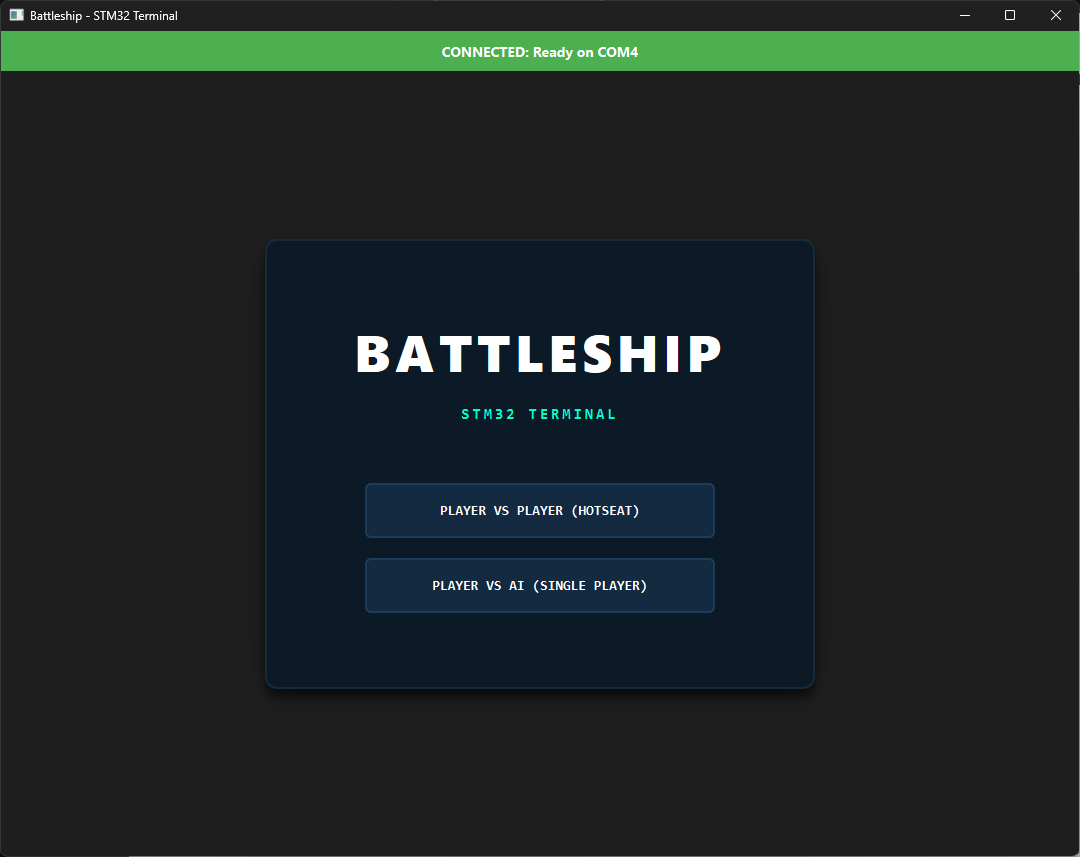
\includegraphics[width=\columnwidth]{figures/image_ai.png}
\caption{PyQt6 GUI client connected to the STM32F051 microcontroller over UART during active Player-vs-AI combat, showing tactical tracking grids, sunk ship alerts, dynamic LED health bar status, and live serial transaction console.}
\label{fig:screenshot}
\end{figure}

\subsection{Empirical Bugs and Lessons Learned}
Hardware testing revealed subtle timing and serialization defects that were undetectable during isolated host mock unit testing:
\begin{enumerate}
    \item \textbf{Premature Frame Timeout on Batch Placement}: The server initially evaluated \texttt{now - last\_rx\_time > FRAME\_TIMEOUT} measured from the \emph{start} of the frame. Because the 53-character \texttt{FLEET} batch command requires more time to serialize across USB CDC buffers when generated slowly by certain host operating systems, frames were occasionally aborted mid-stream. This was resolved by resetting \texttt{last\_rx\_time} on \emph{every received byte} in \texttt{Proto\_ProcessByte()}, converting the mechanism to a genuine inter-byte silence timeout.
    \item \textbf{Host-to-Target CRLF Line Ingestion}: Windows serial drivers emit \texttt{\textbackslash r\textbackslash n} by default. The bare newline parser previously treated \texttt{\textbackslash r} as a coordinate character, causing valid inputs like \texttt{"SHOOT: 1,A1\textbackslash r\textbackslash n"} to fail coordinate boundary conversion. Explicitly ignoring \texttt{0x0D} on byte ingestion permanently eradicated the issue.
    \item \textbf{Interrupt Re-Arming Race Condition}: Calling \texttt{HAL\_UART\_Receive\_IT()} at the very end of \texttt{HAL\_UART\_RxCpltCallback()} occasionally caused an overrun flag (\texttt{ORE}) if a second character arrived during frame dispatch. Relocating the re-arm call immediately after reading \texttt{rx\_byte} eliminated all overrun errors.
\end{enumerate}

\section{Conclusion}
\label{sec:conclusion}

\begin{guidance}[Conclusion (5 marks)]
Summarise \textbf{success} (which requirements you met, with evidence),
\textbf{usefulness} (where this design would apply beyond the project),
\textbf{limitations} (be honest: what does not work, or only works under
conditions) and \textbf{possible improvements}. No new results here.
\end{guidance}

This paper presented the complete engineering realization of an authoritative serial game server and desktop client for Battleship, deployed on the STM32F051R8 ARM Cortex-M0 microcontroller. Every functional requirement specified in the course brief was satisfied in full, validated across 80 automated hardware-in-the-loop tests with 100\% pass rates on physical hardware. The system guarantees absolute server-side authority, strict state invariance under malformed or illegal commands, atomic two-phase fleet placement, deterministic turn alternation, and autonomous on-chip probability heatmap AI combat, accompanied by real-time hardware LED bar-graph and buzzer telemetry.

\textbf{Usefulness.} The design paradigms established in this work generalize directly to mission-critical embedded systems and industrial distributed control applications:
\begin{itemize}
    \item \textbf{Defensive Serial Protocol Engineering}: The combination of newline delimiter synchronization, bounded memory assembly, inter-byte silence timeouts, and atomic multi-tiered parameter validation forms an adaptable template for SCADA, Modbus, and aerospace telemetry links operating across noisy channels.
    \item \textbf{Authoritative State Machine Isolation}: Decoupling untrusted presentation layers from authoritative embedded logic mirrors modern financial transactional terminals, point-of-sale systems, and medical devices where the host PC cannot be trusted with critical state variables.
    \item \textbf{Resource-Constrained Edge Intelligence}: The integer-only probability density search algorithm proves that heuristic computer intelligence can operate deterministically within tightly constrained microcontrollers without floating-point units or operating system runtimes.
\end{itemize}

\textbf{Limitations.} While fully functional and robust against communications anomalies, the current implementation exhibits several engineering constraints:
\begin{enumerate}
    \item \textbf{Point-to-Point Topology}: The architecture relies on a single full-duplex UART interface. In two-player mode, players must operate in a turn-based ``hotseat'' configuration sharing one client instance, rather than connecting separate independent physical consoles.
    \item \textbf{Volatile Game State}: Current game variables and statistics reside strictly in SRAM; disconnecting the board or pressing the hardware reset button clears the active session without persisting match histories or high scores to non-volatile Flash memory.
    \item \textbf{Baud Rate Fixity}: Communication is statically constrained to 115,200\,bps. Dynamic baud-rate negotiation or auto-baud detection is not supported.
\end{enumerate}

\textbf{Improvements.} Future extensions could further expand the embedded server's capabilities:
\begin{enumerate}
    \item \textbf{Dual-Client Networked Play}: Upgrading the physical communication layer to a multi-drop RS-485 bus or implementing a secondary UART channel would allow two independent physical desktop clients to connect concurrently, eliminating hotseat turn sharing while maintaining complete fog-of-war.
    \item \textbf{Non-Volatile Flash Persistence}: Utilizing the STM32F051's internal Flash memory for EEPROM emulation to store lifetime win/loss tallies, match records, and leaderboard statistics across power cycles.
    \item \textbf{Dynamic Turn Timers and Move Clocks}: Incorporating a countdown hardware timer (e.g.\ TIM2) to enforce a per-move time limit, penalizing stalled players with turn forfeiture to accelerate competitive match pace.
\end{enumerate}

\section{Video}
\label{sec:video}

\begin{guidance}[Video (required)]
A short video of \textbf{your group} demonstrating the working STM32 game
server: connect, legal moves, a rejected move, a win or draw, moves disabled
after game over, a new game, the button and LED behaviour, and disconnect.
Show the board and the screen. Check that the link works for someone who is
not logged in as you.
\end{guidance}

The demonstration video is available at:
\begin{center}
\url{https://ssp.faurholm.stream/eee_video.mp4}
\end{center}
The recording demonstrates the STM32F051R8 Discovery board and the PyQt6 client operating in real time: serial handshake negotiation, interactive fleet placement, valid hits and misses with auditory and visual feedback, rejection of out-of-turn and repeat coordinates, hardware 5-LED dynamic health bar tracking on PB3--PB7, board push-button hardware interrupts for immediate game reset, a complete win sequence with opponent fleet coordinate reveal, and graceful post-game disconnect.

\section{Code}
\label{sec:code}

\begin{guidance}[Code (required)]
Link to the GitHub repository with the STM32CubeIDE project, the GUI, the test
harness, and a README with setup, build, flash, run and test instructions.
Before you submit, clone it into a clean folder and follow your own README
(brief, p.~5). Make sure the repository is accessible to the markers.
\end{guidance}

The complete project source code is available on GitHub at:
\begin{center}
\url{https://github.com/frhsco001/EEE3095S-Project}
\end{center}
The repository contains the complete STM32CubeIDE embedded C project (under \texttt{server/}), the PyQt6 desktop client and automated pytest test harness (under \texttt{client/}), and the complete documentation and report source files, complete with comprehensive setup, compilation, flashing, and verification instructions in the root and component \texttt{README.md} files.


\bibliographystyle{IEEEtran}
\bibliography{refs}

\end{document}
